%%% Local Variables:
%%% mode: latex
%%% TeX-master: "../index"
%%% End:

% Recommended:
% Prime generation
% Trial division
% Miller-Rabin
% - Not guaranteed correct, but chance of fault can be made small.

\subsection*{Agenda}
\begin{enumerate}
\item Prime generation
\item Trial division
\item Miller-Rabin
\end{enumerate}

\subsection{Prime Generation}
Primes can be guessed.

We have a method how to approximate number of primes in a interval.
\[ \frac{\pi (m)}{m/\ln m} \]
Here $\pi (m)$ is all primes that are less than $m$.

To generate a $k$-bit prime $m$ we use this approximation to get the
probability of finding $m$. If $m$ lies in the interval $2^{k-1}$ to
$2^k-1$ we get:
\[
\pi (2^k)-\pi (2^{k-1}) \approx
\frac{2^k}{\ln 2^k}-\frac{2^{k-1}}{\ln 2^{k-1}}
\approx \frac{2^{k-1}}{\ln 2^{k-1}}
\]
If we now chose a random m within our interval, we now know what the
probability of it being a prime is. If we exempt all even number, we
increase the probability of guessing the prime with a factor of two.

\subsection{Trial division}
Trial division is quite simple and another way to generate a $k$-bit
prime.
\begin{itemize}
\item input an integer $m$
\item We devide $m$ with all primes $r\le \sqrt{m}$ (This is true since
  if a factor is larger than $\sqrt{m}$ then it has atleast another
  factor that is smaller than $\sqrt{m}$)
\item if $r$ devides $m$ then $m$ isn't prime
\item if all primes $r$ are coprime with $m$ then it is prime
\end{itemize}
This requires that we have all primes under the number we want to find.

\subsection{Miller-Rabin}
Miller-Rabin is another method of determining if a number is prime or
not. It is based on the principles of Fermat's Little Theorem, so in
principle it can rate pseudoprimes as primes, but since the algorithm
runs over multiple iterations, the probability of yielding a
false-positive becomes very small.

When checking for primes we only check odd numbers that are greater
than 2.

\subsubsection*{Principle}
Given an odd number $m$, we start by calculating
\[ m - 1 =2^s t \]

Where $s$ and $t$ are found by subtracting 1 from $m$ and dividing it
by two until result is odd. $s$ is the times we divide by 2 and $t$ is
the odd result.

Now pick a random integer $b$ in the interval $0<b<m$.

\text{With Fermat's Little Theorem} \notag\\
\[ 1 = b^{m-1} \mod m \]
We insert for $m-1$
\[ 0 = b^{2^{s}t}-1\mod m \]
We now expand $b^{2^{s}t} - 1$ by factoring the difference between two squares
\[ 0 = (b^{2^{s-1}t} + 1)(b^{2^{s-1}t} - 1) \mod m \]
We now expand $b^{2^{s-1}t}-1$
\[ 0 = (b^{2^{s-1}t} + 1)(b^{2^{s-2}t} + 1)(b^{2^{s-2}t} - 1) \mod m \]
We keep expanding until $s$ becomes zero
\[ 0 = (b^{2^{s-1}t} + 1)(b^{2^{s-2}t} + 1) \ldots (b^{t} + 1)(b^{t} - 1) \mod m \]

It is known that if $ab \equiv 0 \mod p$ then $a \equiv 0
\mod p$ or $b \equiv 0 \mod p$. Therefore, either
\[ b^{2^{i}t} \equiv -1 \mod p \quad \text{for } i = 0, \ldots, s-1 \]
must hold, or
\[ b^t \equiv 1 \mod p \]
for $m$ to be a \emph{probable} prime.

E.g. if we pretend that $b^{2^{s-1}t} \equiv -1 \mod m$
\begin{align*}
  0 &= (-1+1)(b^{2^{s-2}t}+1)...(b^{2^t}+1)(b^{2^t} - 1) \mod m \\
  0 &= 0 \cdot (b^{2^{s-2}t}+1)...(b^{2t}+1)(b^{2t} - 1) \mod m \\
  0 &= 0 \mod m \\
\end{align*}

\subsubsection*{Algorithm}
\begin{figure}[H]
  \begin{centering}
    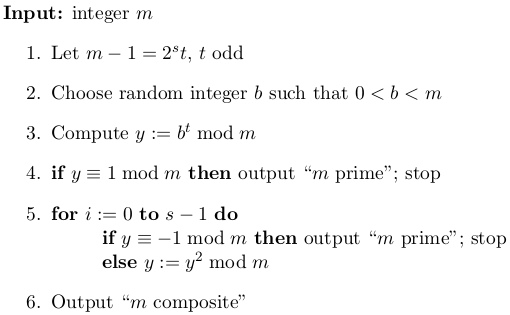
\includegraphics[width=11cm]{images/7-miller-rabin}
    \caption{The Miller-Rabin primality test}
  \end{centering}
\end{figure}

\subsubsection*{Correctness}
Even if the algorithm yields ``prime'' for $m$, we cannot be
completely sure if $m$ really is prime. On the other hand, if it
yields ``composite'', we know that it is \emph{not} a prime.

It can be shown that Miller-Rabin has at most $1/4$ probability of
yielding a false-positive. This can be countered by doing several
iterations with different random values for $b$. This lowers the
chance of the algorithm being wrong by $\frac{1}{4}^l$, where $l$ is
the number of different values for $b$ tested.